\documentclass[epsfig,10pt,fullpage]{article}

\newcommand{\LabNum}{2}
\newcommand{\CommonDocsPath}{../../common/docs}
\addtolength{\textwidth}{1.5in}
\addtolength{\oddsidemargin}{-0.75in}
\addtolength{\topmargin}{-0.75in}
\addtolength{\textheight}{1.5in}
\addtolength{\evensidemargin}{0.75in}
\setlength\parindent{0pt}
\raggedbottom

\usepackage{ae,aecompl}
\usepackage{epsfig,float,times}
\usepackage[hypcap]{caption}
\usepackage[pdftex, colorlinks]{hyperref}
\usepackage{graphicx}
\usepackage[usenames, dvipsnames]{color}
\usepackage{rotating}
\usepackage{tikz}
\usetikzlibrary{automata,positioning}
\usepackage{placeins}

\widowpenalty 10000
\clubpenalty 10000

\newcommand{\red}[1]{{\color{red}\sf{#1}}}
\newcommand{\green}[1]{{\color{green}\sf{#1}}}
\newcommand{\blue}[1]{{\color{blue}\sf{#1}}}
\definecolor{PineGreen}{rgb}{0.0, 0.47, 0.44}
\definecolor{ForestGreen}{rgb}{0.13, 0.55, 0.13}
\definecolor{Brown}{rgb}{0.59, 0.29, 0.0}

\newcommand{\UPDatePublished}{Oct 2021}
\newcommand{\versnum}{21.1} %version number quartus/AMP
\newcommand{\quartusname}{Quartus\textsuperscript{\textregistered} Prime}	
\newcommand{\UPTextBar}{For \quartusname{} \versnum{}}
\newcommand{\thisyear}{2021 } %for copyright
\newcommand{\company}{FPGAcademy.org}
\newcommand{\longteamname}{FPGAcademy.org}
\newcommand{\teamname}{FPGAcademy}
\newcommand{\website}{FPGAcademy.org}

\newcommand{\productAcronym}{AMP}
\newcommand{\productNameShort}{Monitor Program}

\newcommand{\productNameMedTM}{A Monitor Program}
\newcommand{\productNameMed}{A Monitor Program}

%\newcommand{\headerLogoFilePath}[1]{#1/FPGAcademy.png}

% listings is a package that supports encapsulating source code in LaTeX conveniently
\usepackage{listings}

\def\expandparam\lstinputlisting[#1]#2{\edef\tmp{\noexpand\lstinputlisting[#1]{#2}}\tmp}

%%%%%%%%%%%%%%%%%%%% Source Code Formatting %%%%%%%%%%%%%%%%%%%%
\definecolor{globalCommentColour}{rgb}{0.588,0.588,0.588}

%%%%%%%%%%%%%%%%%%%%%%%%%%%%%%%%%%%%%%%%%%%%%%%%%%%%
% Defining language style
% NiosII ASM
\lstdefinelanguage[NiosII]{Assembler} {
  morekeywords={add, addi, and, andhi, andi, beq, bge, bgeu, bgt, bgtu, ble,  bleu, blt, bltu, bne, br, break,
  bret, call, callr, cmpeq, cmpeqi, cmpge, cmpgei, cmpgeu, cmpgeui, cmpgt, cmpgti, cmpgtu, cmpgtui, cmple,
  cmplei, cmpleu, cmpleui, cmplt, cmplti, cmpltu, cmpltui, cmpne, cmpnei, custom, div, divu, eret, flushd,
  flushda, flushi, flushp, initd, initda, initi, jmp, jmpi, ldb, ldbio, ldbu, ldbuio, ldh, ldhio, ldhu, ldhuio,
  ldw, ldwio, mov, movhi, movi, movia, movui, mul, muli, mulxss, mulxsu, mulxuu, nextpc, nop, nor, or, orhi, ori,
  rdctl, rdprs, ret, rol, roli, ror, sll, slli, sra, srai, srl, srli, stb, stbio, sth, sthio, stw, stwio,
  sub, subi, sync, trap, wrctl, wrtcl, wrprs, xor, xori, xorhi, xori},
  morekeywords=[2]{.abort, .ABORT, .align, .app-file, .ascii, .asciz, .balign, .byte, .comm, .data, .def,
  .desc, .dim, .double, .eject, .else, .end, .endef, .endif, .equ, .equiv, .err, .extern, .file, .fill, .float,
  .global, .globl, .hword, .ident, .if, .include, .int, .irp, .irpc, .lcomm, .lflags, .line, .linkonce, .ln,
  .list, .long, .macro, .mri, .nolist, .octa, .org, .p2align, .psize, .quad, .rept, .sbttl, .scl, .section,
  .set, .short, .single, .size, .sleb128, .skip, .space, .stadb, .stabn, .stabs, .string, .symver, .tag,
  .text, .title, .type, .val, .uleb128, .word},
  morekeywords=[3]{et, bt, gp, sp, fp, ea, sstatus, ra, pc, status, estatus, bstatus, ienable, ipending, cpuid,
  exception, pteaddr, tlbacc, tlbmisc, eccinj, badaddr, config, mpubase, mpuacc},
  sensitive=t,
  alsoletter=.,
  morestring=[b]",
  morecomment=[s]{/*}{*/},
  morecomment=[l]\#,
}[keywords,comments,strings]
   
%% NOTE: morekeywords=[2] are GNU directives.
   
\definecolor{niosInstructionColour}{rgb}{0.000,0.608,0.000}
\definecolor{niosDirectiveColour}{rgb}{0.000,0.000,0.902}
\definecolor{niosSpecialRegColour}{rgb}{0.000,0.000,0.000}
\definecolor{niosStringColour}{rgb}{0.808,0.482,0.000}
   
%% NOTE: To make bold use: =\bfseries\color{<colour>}
\lstdefinestyle{defaultNiosStyle} {
  language=[NiosII]{Assembler},
  stringstyle=\color{niosStringColour},
  keywordstyle=\color{niosInstructionColour},
  keywordstyle=[2]\color{niosDirectiveColour},
  keywordstyle=[3]\itshape\color{niosSpecialRegColour}
}
%%%%%%%%%%%%%%%%%%%%%%%%%%%%%%%%%%%%%%%%%%%%%%%%%%%%

%%%%%%%%%%%%%%%%%%%%%%%%%%%%%%%%%%%%%%%%%%%%%%%%%%%%
% Defining language style
% ArmA9 ASM
\lstdefinelanguage[ArmA9]{Assembler} {
  morekeywords={ADC, ADD, ADDS, AND, ANDS, B, BAL, BEQ, BGE, BGT, BL, BLT, BIC, BKPT, BLX, BNE, BX, CDP, CLZ, CMN, CMP, EOR,
  EORS, LDC, LDM, LDR, LDRB, LDRBT, LDRH, LDRSB, LDRSH, LDRT, LSL, MCR, MLA, MOV, MOVW, MOVT, MRC, MRS, MSR, MUL, MVN, ORR, PLD,
  ROR, RSB, RSC, SBC, SMLAL, SMULL, STC, STM, STR, STRB, STRBT, STRH, STRT, SUB, SUBS, SWI, SWP, SWPB, TEQ, UMLAL,
  PUSH, POP, MOVS, RORS, LSR},
  morekeywords=[2]{.abort, .ABORT, .align, .app-file, .ascii, .asciz, .balign, .byte, .comm, .data, .def,
  .desc, .dim, .double, .eject, .else, .end, .endef, .endif, .equ, .equiv, .err, .extern, .file, .fill, .float,
  .global, .globl, .hword, .ident, .if, .include, .int, .irp, .irpc, .lcomm, .lflags, .line, .linkonce, .ln,
  .list, .long, .macro, .mri, .nolist, .octa, .org, .p2align, .psize, .quad, .rept, .sbttl, .scl, .section,
  .set, .short, .single, .size, .sleb128, .skip, .space, .stadb, .stabn, .stabs, .string, .symver, .tag,
  .text, .title, .type, .val, .vectors, .uleb128, .word},
  morekeywords=[3]{SP, PC, MIDR, CTR, TCMTR, TLBTR, MPIDR, ID_PFR0, ID_PFR1, ID_DFR0, ID_MMFR0, ID_MMFR1, ID_MMFR2,
  ID_MMFR3, ID_ISAR0, ID_ISAR1, ID_ISAR2, ID_ISAR3, ID_ISAR4, CCSIDR, CLIDR, AIDR, CSSELR, TTBR0, TTRB1, TTBR2, DACR,
  DFSR, IFSR, ADFSR, AIFSR, DFAAR, IFAR, ICIALLUIS, BPIALLIS, PAR, ICIALLU, ICIMVAU, BPIALL, DCIMVAC, DCISW, V2PCWPR,
  DCCVAC, DCCSW, DDIMVAC, DCISW, TLBALLIS, TLBIMVAIS, TLBIASIDIS, TLBIMVAAIS, TLBIALL, TLBIMVA, TLBIASID, TLBIMVAA,
  PMCR, PMCNTENSET, PMCNTENCLR, PMOVSR, PMSWINC, PMSELR, PMXEVTYPER, PMXEVCNTR, PMUSERENR, PMINTENSET, PMINTENCLR,
  PRRR, NRRR, PLEIDR, PLEASR, PLEFSR, PLEUAR, PLEPCR, VBAR, MVBAR, ISR, FCSEIDR, CONTEXTIDR, TPIDRURW, TPIDRURO, TPIDRPRW},
  sensitive=f,
  alsoletter=.,
  morestring=[b]",
  morecomment=[s]{/*}{*/},
  morecomment=[l]{//},
}[keywords,comments,strings]
   
%% NOTE: morekeywords=[2] are GNU directives.
   
\definecolor{armInstructionColour}{rgb}{0.000,0.608,0.000}
\definecolor{armDirectiveColour}{rgb}{0.000,0.000,0.902}
\definecolor{armSpecialRegColour}{rgb}{0.000,0.000,0.000}
\definecolor{armStringColour}{rgb}{0.808,0.482,0.000}
   
\lstdefinestyle{defaultArmStyle} {
  language=[ArmA9]{Assembler},
  stringstyle=\color{armStringColour},
  keywordstyle=\color{armInstructionColour},
  keywordstyle=[2]\color{armDirectiveColour},
  keywordstyle=[3]\itshape\color{armSpecialRegColour}
}
%%%%%%%%%%%%%%%%%%%%%%%%%%%%%%%%%%%%%%%%%%%%%%%%%%%%

%%%%%%%%%%%%%%%%%%%%%%%%%%%%%%%%%%%%%%%%%%%%%%%%%%%%
% Defining language style
% FPGAcademy ASM
\lstdefinelanguage{ASM}{
  morekeywords = [1]{mv, mvt, mvne, mvcc, add, sub, st, ld, and, b, bne, beq, bcc, bcs},
  morekeywords = [2]{word, define},
  keywordstyle = [1]\color{ForestGreen},
  keywordstyle = [2]\color{blue},
  sensitive = true,
  morecomment = [l]{//},
}

\lstset{
  language = ASM,
  basicstyle=\small\color{black}\ttfamily,
  commentstyle=\small\color{Brown}\itshape\ttfamily,
  showstringspaces=false,
  frame=none, %lines % boxed listings
  breaklines=true,
  breakatwhitespace=true,
  tabsize=3
}
%%%%%%%%%%%%%%%%%%%%%%%%%%%%%%%%%%%%%%%%%%%%%%%%%%%%

%%%%%%%%%%%%%%%%%%%%%%%%%%%%%%%%%%%%%%%%%%%%%%%%%%%%
% Defining language style
% Java
\definecolor{javaStringColour}{rgb}{0.808,0.482,0}
%%%%%%%%%%%%%%%%%%%%%%%%%%%%%%%%%%%%%%%%%%%%%%%%%%%%

%%%%%%%%%%%%%%%%%%%%%%%%%%%%%%%%%%%%%%%%%%%%%%%%%%%%
% Defining language style
% C
\definecolor{CStringColour}{rgb}{0.808,0.482,0}

\lstset{
  language = C,
  basicstyle=\small\color{black}\ttfamily, 
  commentstyle=\small\color{PineGreen}\itshape\ttfamily,
  keywordstyle=\small\color{blue}\bfseries\ttfamily,
  showstringspaces=false,
  frame=none, %lines % boxed listings
  breaklines=true,
  breakatwhitespace=true,
  tabsize=3
}
%%%%%%%%%%%%%%%%%%%%%%%%%%%%%%%%%%%%%%%%%%%%%%%%%%%%

%%%%%%%%%%%%%%%%%%%%%%%%%%%%%%%%%%%%%%%%%%%%%%%%%%%%
% Defining language style
% Verilog
\definecolor{verilogCommentColour}{rgb}{0.000,0.502,0.000}

\lstdefinestyle{defaultVerilogStyle} {
  language={Verilog},
  keywordstyle=\color{blue},
  commentstyle=\color{verilogCommentColour}
}
%%%%%%%%%%%%%%%%%%%%%%%%%%%%%%%%%%%%%%%%%%%%%%%%%%%%

%%%%%%%%%%%%%%%%%%%%%%%%%%%%%%%%%%%%%%%%%%%%%%%%%%%%
% Defining language style
% VHDL
\lstdefinestyle{defaultVHDLStyle} {
  language={VHDL},
  keywordstyle=\color{blue},
  commentstyle=\color{verilogCommentColour}
}
%%%%%%%%%%%%%%%%%%%%%%%%%%%%%%%%%%%%%%%%%%%%%%%%%%%%

%%%%%%%%%%%%%%%%%%%%%%%%%%%%%%%%%%%%%%%%%%%%%%%%%%%%
% Defining language style
% LaTeX
\lstdefinelanguage[LocalLaTeX]{TeX}[LaTeX]{TeX}{moretexcs={bf, it, sf, lstset},}

\lstdefinestyle{defaultLocalLatexStyle} {
  language=[LocalLatex]{TeX},
  keywordstyle=\color{blue}\bfseries,
  keywordstyle=[2]\color{blue},
  keywordstyle=[3]\color{blue}\bfseries
}
%%%%%%%%%%%%%%%%%%%%%%%%%%%%%%%%%%%%%%%%%%%%%%%%%%%%

%%%%%%%%%%%%%%%%%%%%%%%%%%%%%%%%%%%%%%%%%%%%%%%%%%%%
% Defining language style
% Default
\lstset{
  basicstyle=\small\color{black}\ttfamily,
  commentstyle=\small\color{globalCommentColour}\itshape\ttfamily,
  keywordstyle=\small\color{blue}\bfseries\ttfamily,
  showstringspaces=false,
  frame=none, %lines % boxed listings
  breaklines=true,
  breakatwhitespace=true,
  tabsize=3
}
%%%%%%%%%%%%%%%%%%%%%%%%%%%%%%%%%%%%%%%%%%%%%%%%%%%%


\hypersetup{
  pdftitle={OpenCL Lab Exercise \LabNum},
  linkcolor=blue,
  hyperindex=true,
  pdfauthor={FPGAcademy.org},
  pdfkeywords={FPGAcademy.org, FPGAcademy, Lab, Exercise, OpenCL},
  bookmarks,
  bookmarksopen=false,
  filecolor=blue,
  pdfstartview={FitH},
  urlcolor=blue,
  plainpages=false,
  pdfpagelabels=true,
  linkbordercolor={1 1 1} %no color for link border
}



\begin{document}

\centerline{\huge OpenCL}
~\\
\centerline{\huge Laboratory Exercise \LabNum}
~\\
\centerline{\large Accelerating Computer Vision Techniques}
~\\

This exercise introduces you to accelerating computer vision techniques using the Intel FPGA SDK for OpenCL. 

\section*{The Canny Edge-detection Technique}

\noindent
In this exercise, we will implement a variation of the \textit{Canny edge detector}, which is 
a widely-used edge-detection scheme in computer vision applications. Figures~\ref{fig:tracks} and \ref{fig:tracks_edges} 
show a sample image that is provided as the input to a Canny edge detector, as well as the 
resulting edge-detected output image. 

~\\
\noindent
The Canny edge-detection algorithm involves five stages which are applied to the input image in 
succession. The details of these stages are given below. As well, we will see how the sample 
input image from Figure~\ref{fig:tracks} is transformed as it passes through 
each stage.

~\\
~\\
\begin{figure}[h]
\centering
\begin{minipage}[b]{0.475\textwidth}
	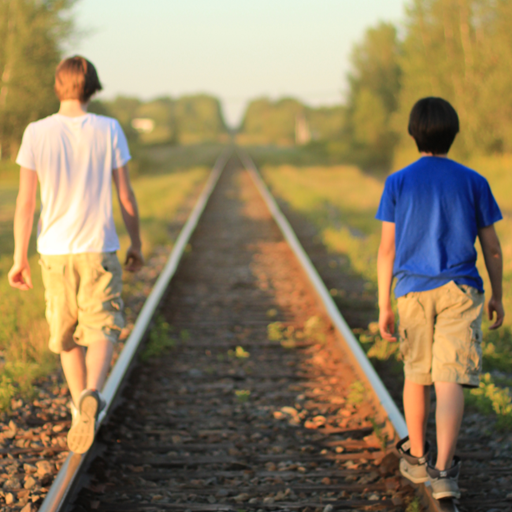
\includegraphics[width=\textwidth]{figures/tracks.png}
	\caption{Original image.}
	\label{fig:tracks}
\end{minipage}
\hfill
\begin{minipage}[b]{0.475\textwidth}
	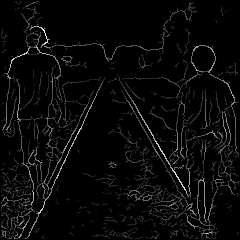
\includegraphics[width=\textwidth]{figures/tracks_edges.png}
	\caption{Edge-detected image.}
	\label{fig:tracks_edges}
\end{minipage}
\end{figure}

\pagebreak

\noindent
\section*{Stage 1: Grayscale Conversion}

Figure~\ref{fig:sample_stage1} shows the state of our sample image at the end of the grayscale 
conversion stage. This stage converts the input 24-bit bitmap color image (8 bits each for red, 
green, and blue) into an 8-bit grayscale image. The grayscale value at each pixel is calculated 
as the average of the three 8-bit color values of the original image.

\begin{figure}[H]
   \begin{center}
       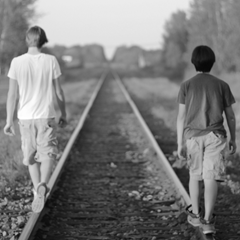
\includegraphics[scale = 0.85]{figures/fig_stage1_grayscale.png}
   \end{center}
   \caption{The sample input image after the grayscale conversion stage.}
	\label{fig:sample_stage1}
\end{figure}

\noindent
\section*{Stage 2: Gaussian Smoothing}

Figure~\ref{fig:sample_stage2} shows the state of our sample image at the end of the gaussian 
smoothing stage. In this stage, a gaussian filter is used to smooth out the image, by 
modifying noisy pixels (pixels that are unlike their neighbouring pixels) to be more like 
their neighbours. Shown below is the 5 x 5 gaussian filter operation that is applied to the 
image. Note that the * denotes convolution, A is the original image, and B is the resulting 
filtered image. The effect of this operation is that each pixel gets assigned the weighted 
average value of the 5 x 5 grid of pixels surrounding each pixel.

\[
B = 1/159
\begin{bmatrix}
    2 & 4 & 5 & 4 & 2 \\
    4 & 9 & 12 & 9 & 4 \\
    5 & 12 & 15 & 12 & 5 \\
    4 & 9 & 12 & 9 & 4 \\
    2 & 4 & 5 & 4 & 2
\end{bmatrix} * A
\]

\begin{figure}[H]
   \begin{center}
       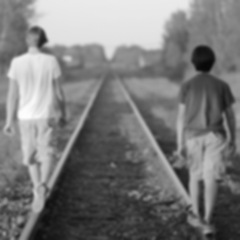
\includegraphics[scale = 0.85]{figures/fig_stage2_gaussian.png}
   \end{center}
   \caption{The sample input image after the gaussian smoothing stage.}
	\label{fig:sample_stage2}
\end{figure}

\noindent
\section*{Stage 3: Sobel Operator} 

Figure~\ref{fig:sample_stage3} shows the state of our sample image at the end of the sobel operator stage. This stage overwrites each pixel with the overall intensity gradient at that pixel. To calculate the overall intensity gradient, the gradient is first calculated in the horizontal ($C_x$) and vertical ($C_y$) directions across the pixel, using the matrices below:

\[
C_x = 
\begin{bmatrix}
    -1 & 0 & 1  \\
    -2 & 0 & 2  \\
    -1 & 0 & 1 
\end{bmatrix} * B
\ \ \ \ \ \ \  \ \ \ \ \  C_y = 
\begin{bmatrix}
    -1 & -2 & -1 \\
    0 & 0 & 0 \\
    1 & 2 & 1
\end{bmatrix} * B
\]

~\\
\noindent
The magnitudes of the two gradients are then added to calculate the overall gradient intensity value for each pixel, resulting in the image C:

\[
C = 0.5|C_x| + 0.5|C_y|
\]

~\\
\noindent
In image C, which is the final output of this stage, the edges of the original image are highlighted as brighter pixels. Non-edges, which are areas with low intensity gradients, appear as darker pixels.

~\\
~\\
\begin{figure}[H]
   \begin{center}
       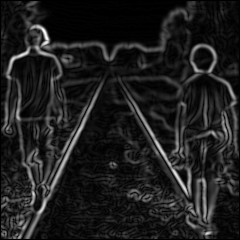
\includegraphics[scale = 0.85]{figures/fig_stage3_sobel.png}
   \end{center}
   \caption{The sample input image after the sobel operator stage.}
	\label{fig:sample_stage3}
\end{figure}

~\\
\noindent
To illustrate the effect of the sobel operator, let us examine different image boundaries that may exist in an image as shown in Figure~\ref{fig:image_boundaries}. For each 3 x 3 image shown, we can use the sobel operator to calculate the intensity gradient at the center pixel. Let us examine the vertical boundary example, where there is a boundary between darker pixels on the left side of the image, and brighter pixels on the right side. In this example, $|C_x|$ of the center pixel can be calculated as |\{-1*2 + 0*98 + 1*181\} + \{-2*1 + 0*94 + 2*178\} + \{-1*6 + 0*91 + 1*184\}| = 711. In the vertical direction, $|C_y|$ for this pixel is calculated to be 7. The intensity gradient for this pixel is high in the horizontal direction, and low in the vertical direction, which is to be expected along a vertical boundary. The total intensity gradient for this pixel, is $0.5*711 + 0.5*7 = 359$ which saturates the 8-bit grayscale channel to value 255. The sobel operator would therefore detect this boundary as a strong edge, and the center pixel would become bright with a value of 255.

\begin{figure}[H]
   \begin{center}
       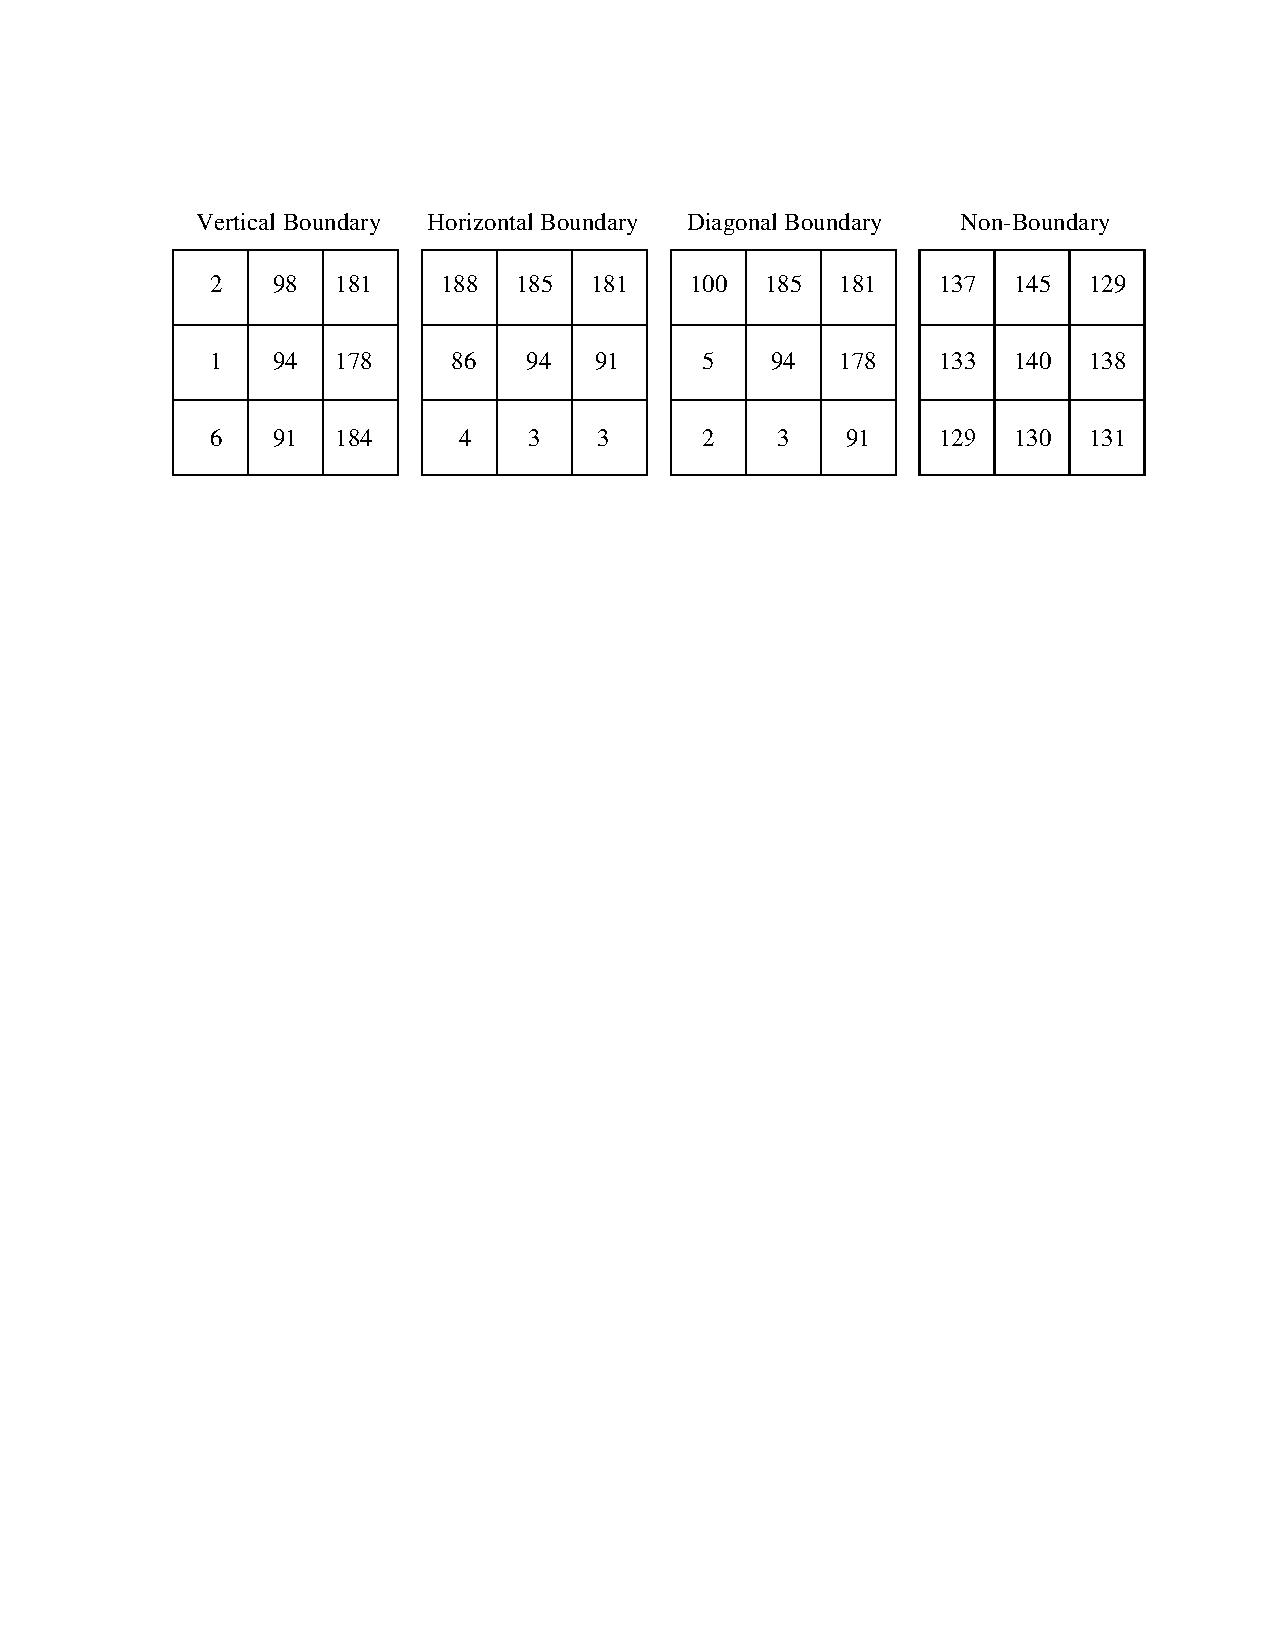
\includegraphics[scale = 0.80]{figures/fig_image_boundaries.pdf}
   \end{center}
   \caption{Examples of boundaries in an image.}
	\label{fig:image_boundaries}
\end{figure}

~\\
\noindent
In the horizontal boundary case, we see that the vertical gradient is high ($|C_y|$ = 726) and the horizontal gradient is low ($|C_x|$ =  2). For the diagonal boundary case, the gradient is high in both directions with $|C_x|$ = 516 and $|C_y|$ = 552. Finally, for the non-boundary case, the gradients are low in both directions with $|C_x|$ = 4 and $|C_y|$ = 36. As the gradients are low, the center pixel would become dark with a value of $0.5*4 + 0.5*36 = 20$.

\noindent
\section*{Stage 4: Non-Maximum Suppression} 

\noindent
Figure~\ref{fig:sample_stage4} shows the state of our sample image at the end of the non-maximum suppression stage. This stage aims to thin the thick and/or blurry edges that may have resulted from the sobel operator stage. Thick edges are problematic as many applications of edge detection benefit from the edges being as thin as possible. For example, to accurately calculate the surface area of an object, thin edges are desired as to not overlap with the surface. The non-maximum suppression stage thins the edges by removing the weaker (non-maximum) pixels of each edge, and keeping only the maxima. Figure~\ref{fig:nonmaximum_suppression} shows the effect of non-maximum suppression on a sample image containing a blurry vertical line. Notice that the vertical line, which is originally three-pixels wide, becomes one-pixel wide.  

~\\
~\\
\begin{figure}[H]
   \begin{center}
       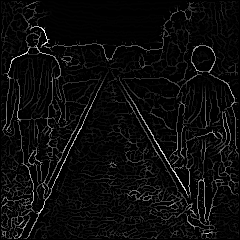
\includegraphics[scale = 0.85]{figures/fig_stage4_nonmax_suppression.png}
   \end{center}
   \caption{The sample input image after the non-maximum suppression stage.}
	\label{fig:sample_stage4}
\end{figure}

\begin{figure}[H]
   \begin{center}
       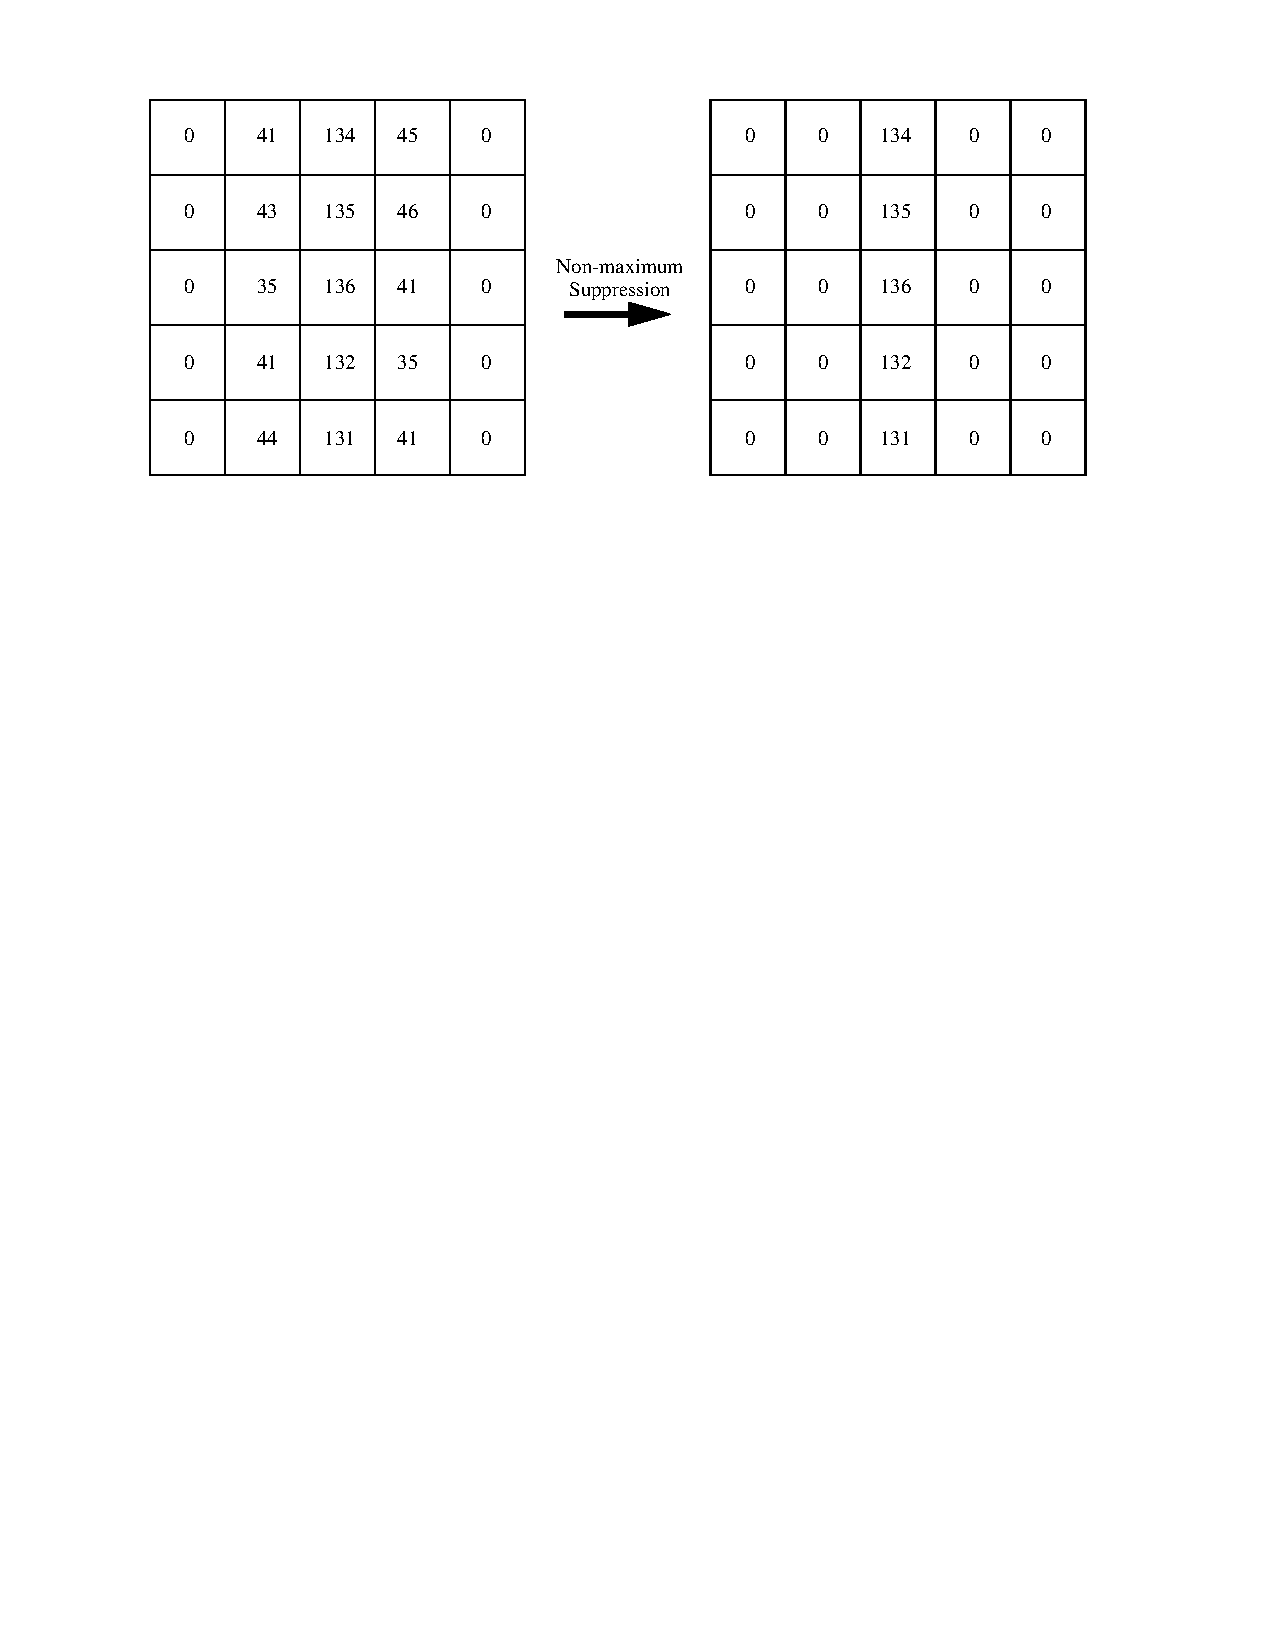
\includegraphics[scale = 0.8]{figures/fig_nonmaximum_suppression.pdf}
   \end{center}
   \caption{The effect of nonmaximum suppression on a blurred vertical line.}
	\label{fig:nonmaximum_suppression}
\end{figure}

\noindent
\section*{Stage 5: Hysteresis}

Figure~\ref{fig:sample_stage5} shows the end result of the hysteresis stage. The goal of the hysteresis stage is to remove pixels that do not belong to an edge and weak edges altogether. This stage uses two user-defined thresholds: the high threshold and the low threshold. The hysteresis algorithm examines each pixel to determine whether: 

\begin{enumerate}
\item the pixel exceeds the high threshold, or
\item the pixel exceeds the low threshold value and there exists at least one adjacent pixel (horizontally, vertically, or diagonally) that exceeds the high threshold.
\end{enumerate}

If at least one of the two criteria are met, the pixel is preserved. Otherwise, the pixel is removed by turning it black.
 
~\\
~\\
\begin{figure}[H]
   \begin{center}
       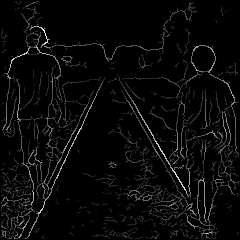
\includegraphics[scale = 0.85]{figures/fig_stage5_hysteresis.png}
   \end{center}
   \caption{The sample input image after the hysteresis stage.}
	\label{fig:sample_stage5}
\end{figure}

\newpage
\section*{Part I}

Write a C++-language program that implements the five stages of the canny edge detector as described in the preceding sections. Start with the skeleton code provided in \textit{/design\_files/part1/}, which contains functionality for loading and storing 24-bit color BMP image files. Once a 24-bit color image is loaded into memory, your code should transform the pixels according to the five stages, then store the resulting edge-detected image. The skeleton also contains code that measures the runtime of your program, which we will use to compare with the OpenCL version. Test your program on the sample BMP 
images provided in \textit{/design\_files/}

\section*{Part II}

Before we proceed with implementing a Canny edge detector using OpenCL, let us devise an efficient memory architecture for
storing the pixel values as they undergo transformations at each Canny stage. Recall that you have two types of memory at your disposal: global memory outside 
the FPGA, and local memories inside the FPGA. The host program provides input data to the accelerator by placing it in global memory.
Since global memory accesses are slow, your accelerator should cache the required pixels into local memory before using them.
The question then, is how to configure the FPGA's local memory resources to best cache the pixels. 

To determine the best memory configuration, let us consider the pixel usage pattern for box operations.
Note that the Gaussian smoothing, Sobel operator, non-max suppression, and hysteresis stages of the detector are all 
types of box operations, as they work on a box (or frame) of pixels to determine each output pixel. 
Figure~\ref{fig:box_operation} depicts a 3x3 box operation (such as the 3x3 sobel operation) on three adjacent pixels of a 10-pixel-wide image. 
Notice that there is significant overlap (6 pixels) in the frames of successive operations.

\begin{figure}[H]
   \begin{center}
       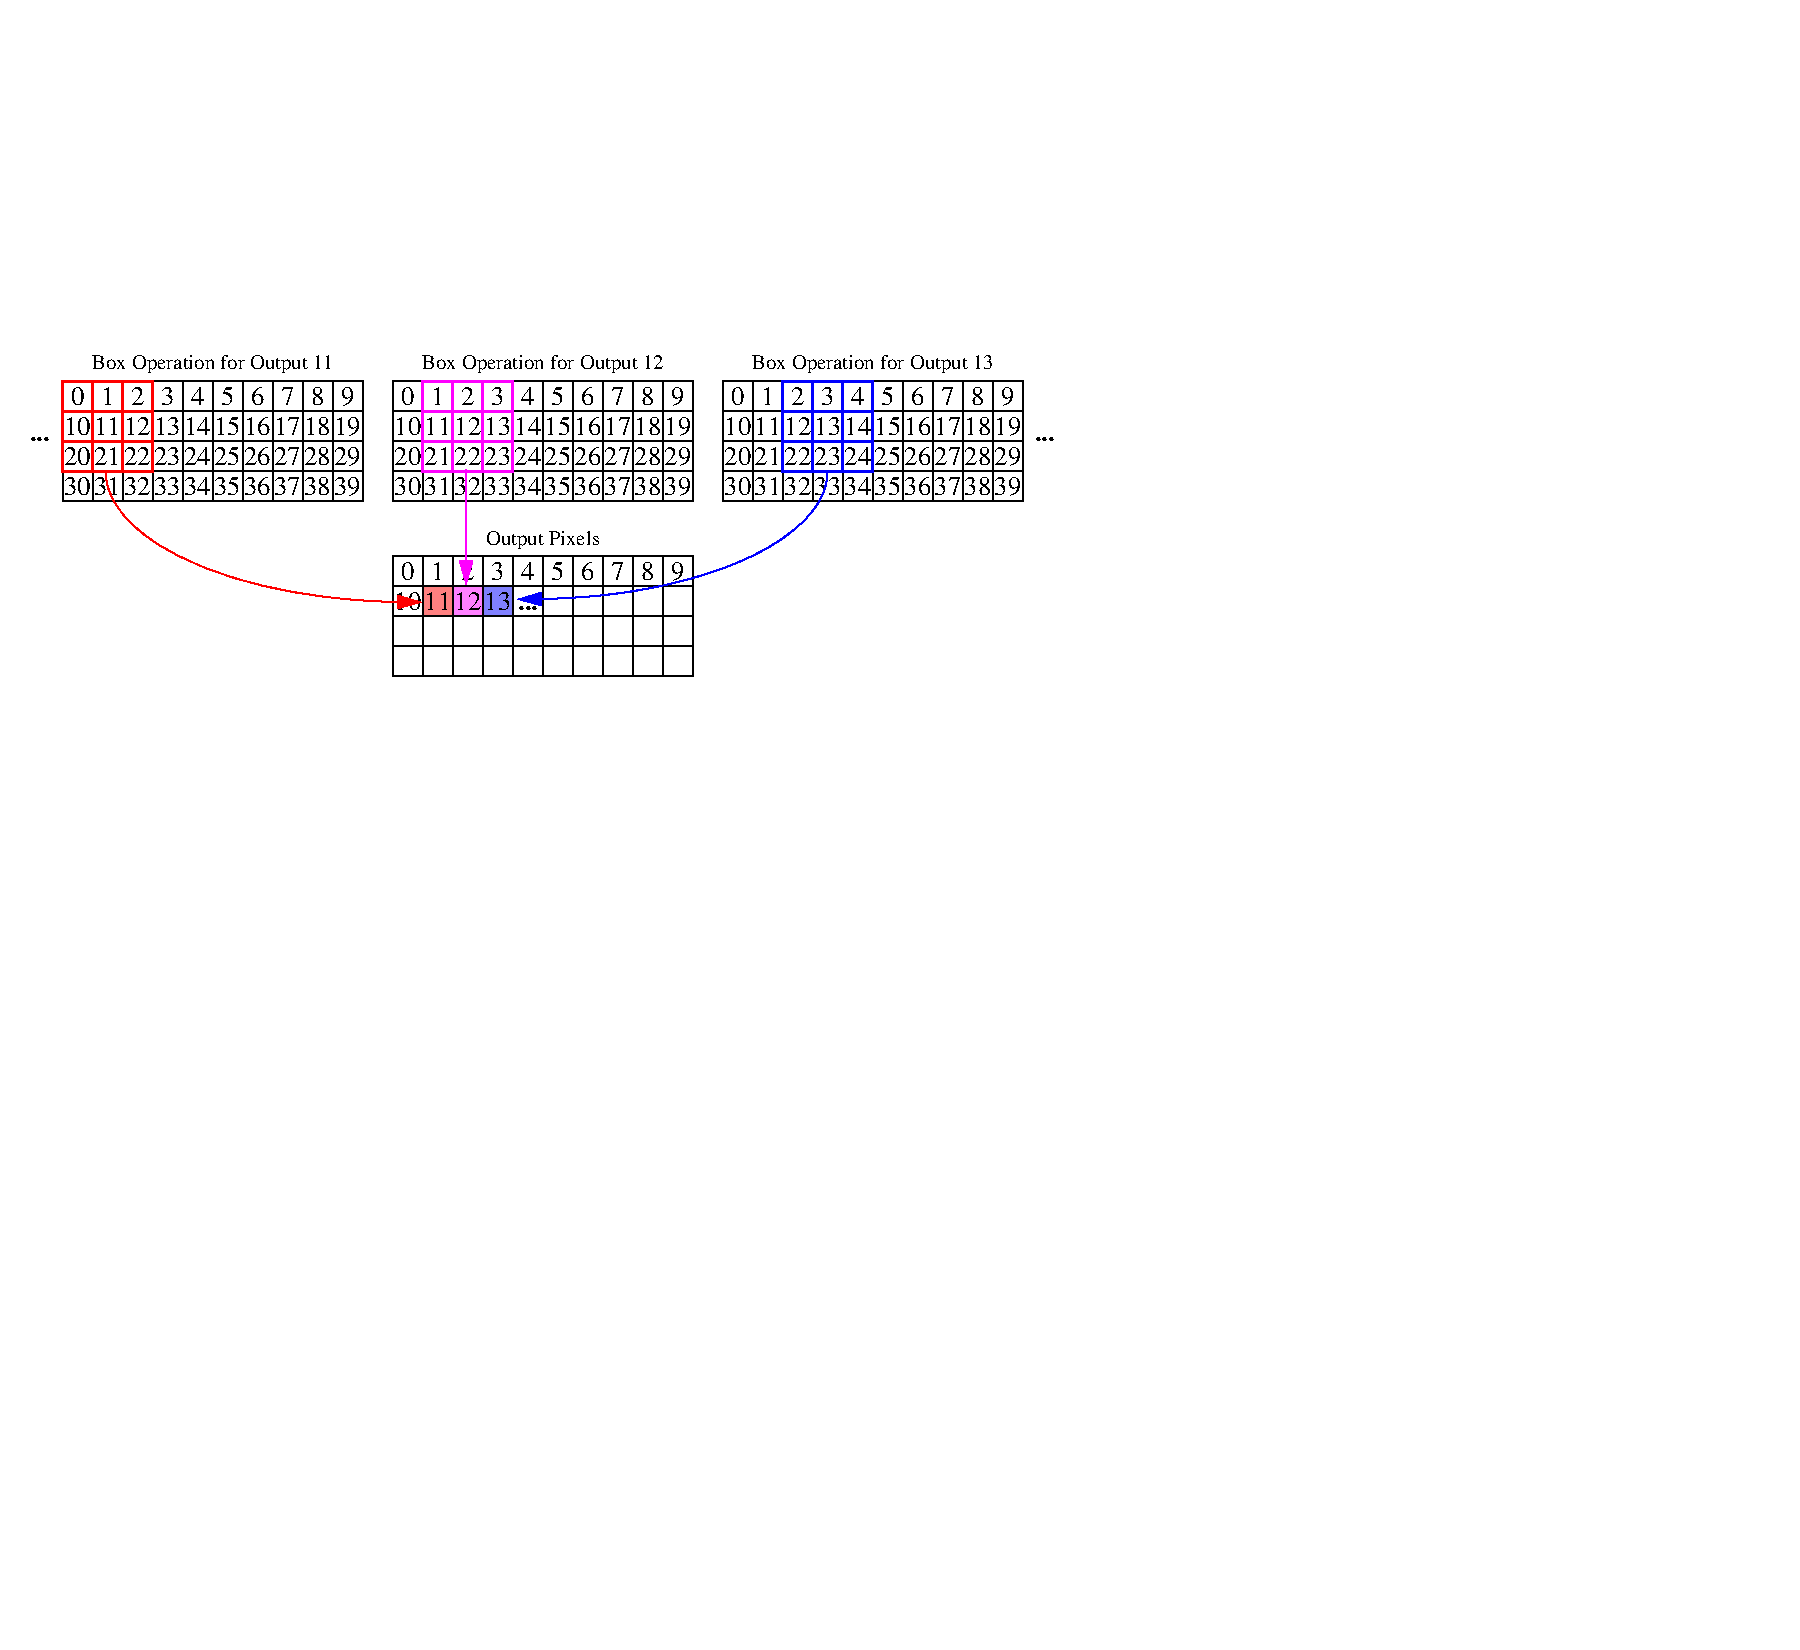
\includegraphics[scale = 0.85]{figures/fig_box_operation}
   \end{center}
   \caption{A 3x3 box operation on three adjacent pixels of a 10-pixel-wide image.}
	\label{fig:box_operation}
\end{figure}

To take advantage of the overlap in successive frames of box operations, we will use the FPGA's local memory resources to construct 
the shift register design shown in Figure~\ref{fig:shift_register}. The figure shows the shift register design for a 3x3 box operation that
works on 10-pixel wide images, but the idea can be extended for arbitrary box sizes and image widths.
Once a sufficient number of pixels have been loaded, the shift register provides a new 3x3 frame for the box operation at every cycle by simply
shifting in a new pixel and shifting out the oldest pixel which is no longer be used.

\begin{figure}[H]
   \begin{center}
       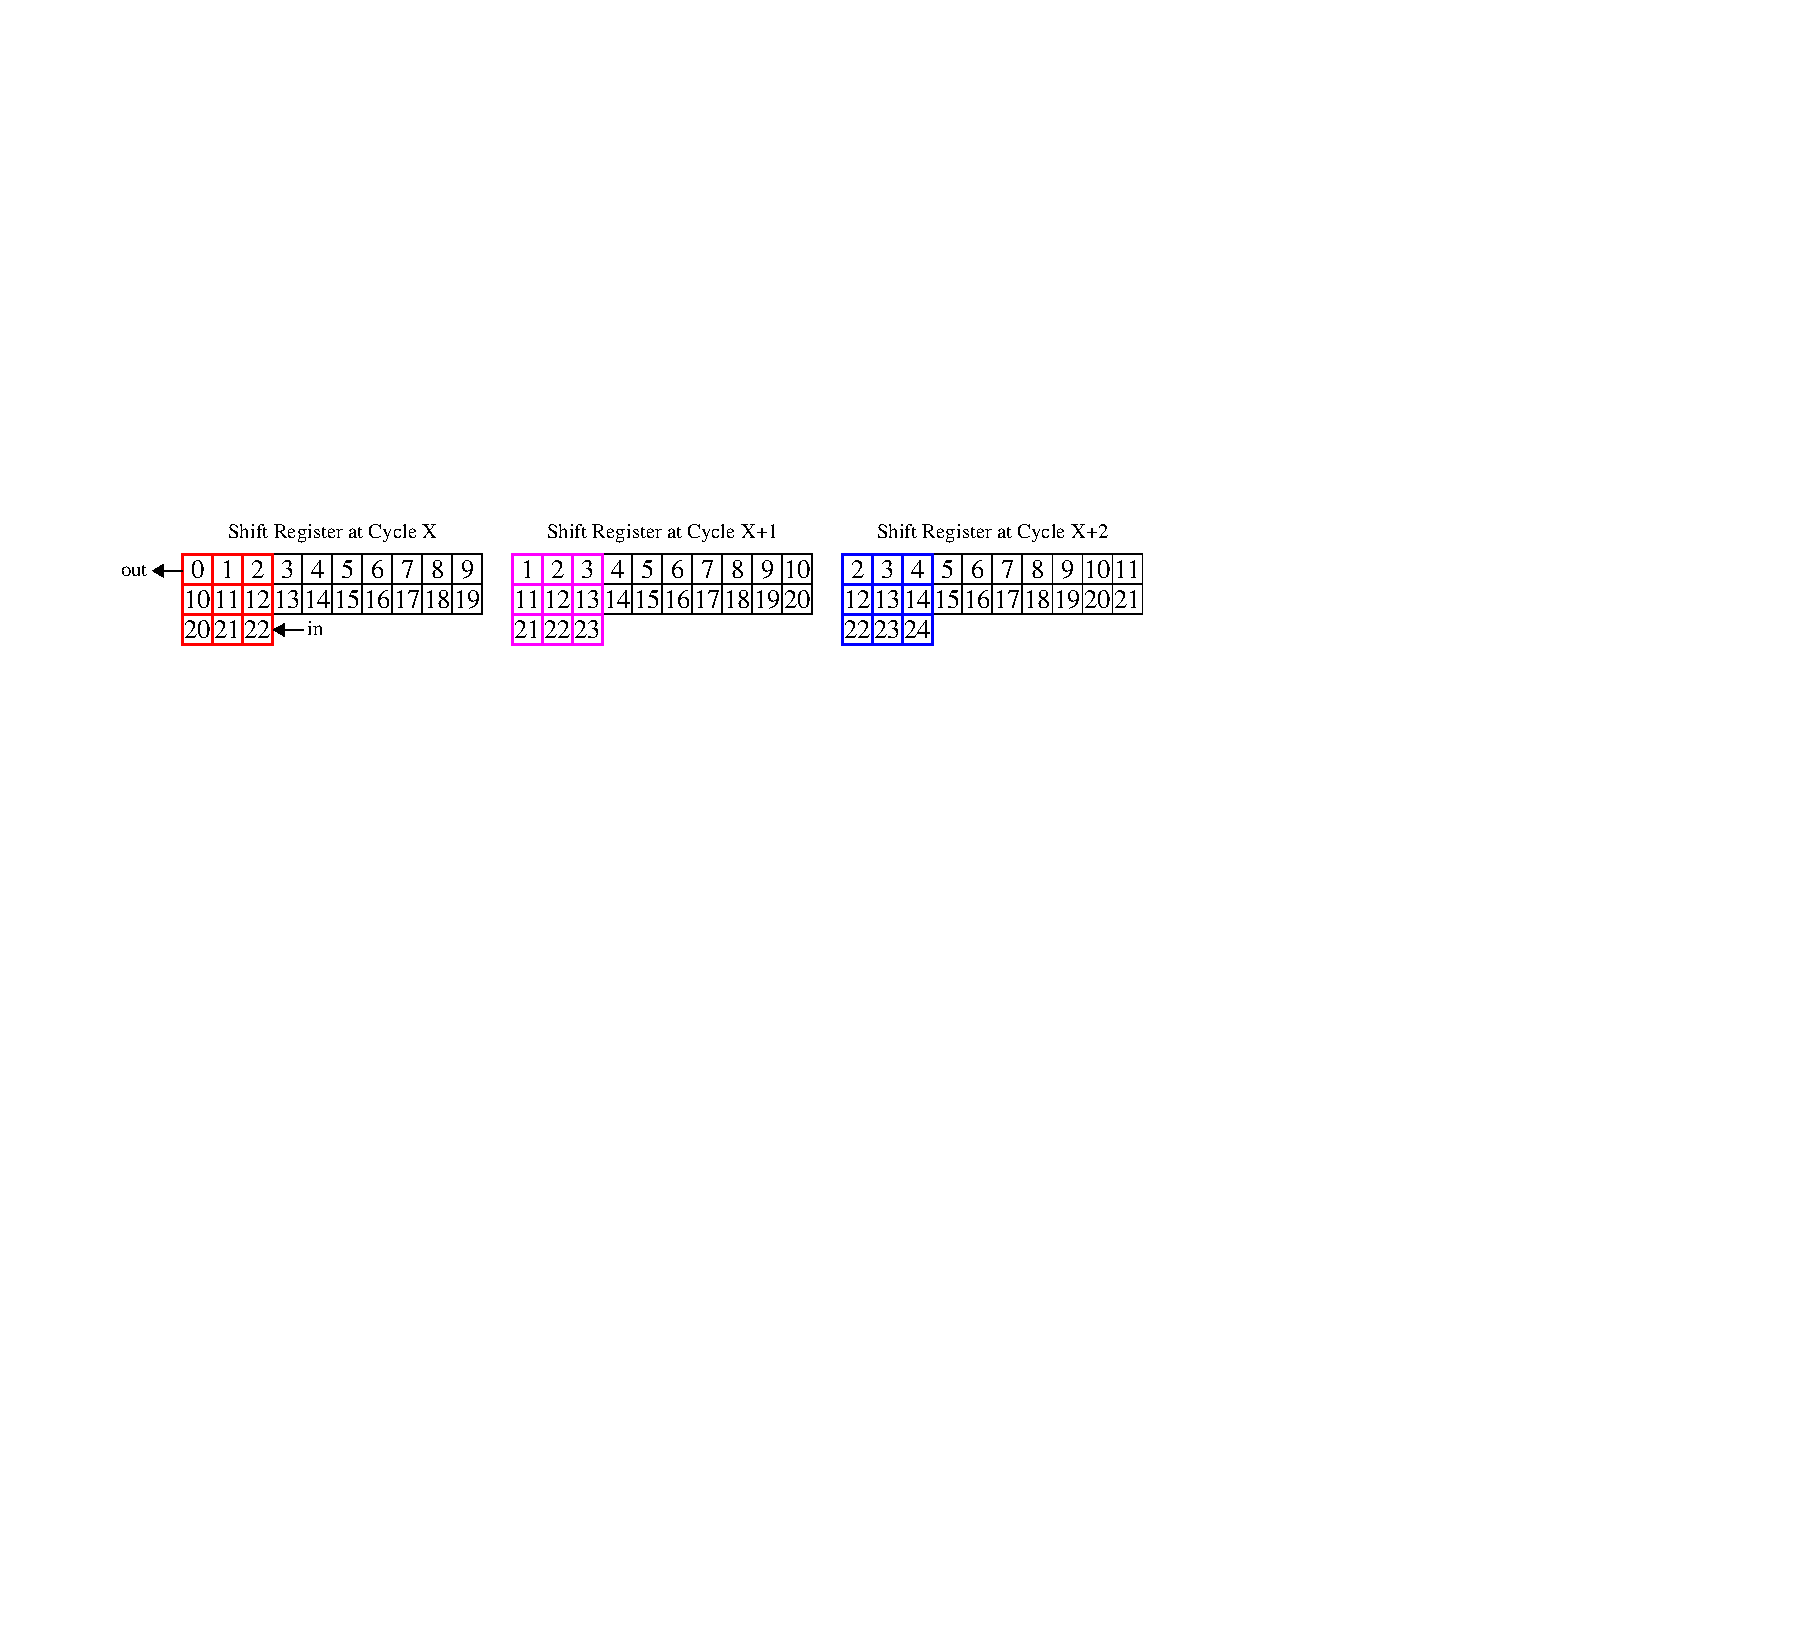
\includegraphics[scale = 0.85]{figures/fig_shift_register}
   \end{center}
   \caption{The shift register for 3x3 box operations on 10-pixel wide images providing 3 frames over 3 cycles.}
	\label{fig:shift_register}
\end{figure}

How many shift registers will you require for your canny edge detector? How large should each of these shift registers be, given that
your circuit works on images that are 720 pixels wide? How many pixels must be loaded into each shift register before the corresponding box operation
can start? Using such a shift register design requires you to zero pad the input image before 
shifting in its pixels, to properly operate on the boundaries of the image. 
Why is zero padding necessary, and what is the necessary padding size for a given box size?


\section*{Part III}

Create an OpenCL application that implements the five stages of the canny edge detector.
Use shift registers to hold the pixels as they undergo the Canny stages, and apply the box operations on the pixels
while they are in flight through the shift registers. The shift registers should be the minimum length necessary to hold
required pixels.
When operating in its steady state, your accelerator should have a throughput of one pixel per clock cycle.
The accelerator is considered to be in its steady state when its shift registers are full. 
For simplicity, do not zero pad the boundaries of the input image and accept some error along the boundary edge pixels.
Your application must be able to operate on images that are 720 pixels wide with variable height.
Start with the skeleton code provided in \textit{/design\_files/part3/}.

~\\
The shift-register design methodology requires the use of Intel FPGA SDK for OpenCL's ability to infer shift registers from 
your OpenCL code. This feature is described in Section \textit{Inferring a Shift Register} of the document \textit{Intel FPGA SDK for OpenCL Programming Guide}.


%%%%%%%%%%%%%%%%%%%%%%%%%%%%%%%%%%%%%%%%
%%% FPGAcademy Copyright Information %%%
%%%%%%%%%%%%%%%%%%%%%%%%%%%%%%%%%%%%%%%%

%Always put the copyright on a new page (clear page), with some vertical space from top
\clearpage
\vspace{1in}

\noindent

Copyright {\copyright} FPGAcademy.org. All rights reserved. FPGAcademy and the 
FPGAcademy logo are trademarks of FPGAcademy.org.  This document is provided 
"as is", without warranty of any kind, express or implied, including but not 
limited to the warranties of merchantability, fitness for a particular purpose 
and noninfringement. In no event shall the authors or copyright holders be 
liable for any claim, damages or other liability, whether in an action of 
contract, tort or otherwise, arising from, out of or in connection with the 
document or the use or other dealings in the document.
~\\
~\\
**Other names and brands may be claimed as the property of others.


\end{document}
